\documentclass{article}

\usepackage[T1]{fontenc}
\usepackage[UTF8]{inputenc}
\usepackage[polish]{babel}
\usepackage{enumitem}
\usepackage{tabulary}
\usepackage{multirow}
%\usepackage{array}
\usepackage{graphicx}
\usepackage{colortbl}
\usepackage{listings}
\usepackage{color}

\definecolor{gray}{rgb}{0.4,0.4,0.4}
\definecolor{darkblue}{rgb}{0.0,0.0,0.6}
\definecolor{cyan}{rgb}{0.0,0.6,0.6}

\lstset{
  basicstyle=\ttfamily,
  columns=fullflexible,
  showstringspaces=false,
  commentstyle=\color{gray}\upshape
}

\lstdefinelanguage{XML}
{
  morestring=[b]",
  morestring=[s]{>}{<},
  morecomment=[s]{<?}{?>},
  stringstyle=\color{black},
  identifierstyle=\color{darkblue},
  keywordstyle=\color{cyan},
  morekeywords={xmlns,version,type}% list your attributes here
}

\let\oldsection\section
\renewcommand\section{\clearpage\oldsection} %break after every section

\definecolor{hlinecolor}{gray}{0.8}
\lstset{
	language=XML,
	morekeywords={encoding,
	}
}


\begin{document}
\title{\textbf{Projekt Zespołowy}\\Moduł generowania pojazdów i map\\z plików graficznych}
\author{Wojciech Kowalik, Konrad Miśkiewicz, Mateusz Pielat}
\maketitle



\tableofcontents


\section{Streszczenie}
Projekt ma na celu stworzenie aplikacji symulującej ruch pojazdu w labiryncie. Pojazd będzie omijał przeszkody poruszając się do przodu i wykonując skręty w miejscu. Aplikacja będzie podzielona na kilka podstawowych modułów, które razem umożliwią przygotowanie i przeprowadzenie symulacji.
\\\\Dokument opisuje technologie oraz rozwiązania zastosowane przy implementacji modułu generowania pojazdów i map z plików graficznych. Moduł ten umożliwia użytkownikowi załadowanie pliku graficznego w jednym z dozwolonych formatów, a następnie jego trasowanie. Użytkownik otrzymuje listę wygenerowanych wielokątów, z których następnie może stworzyć mapę lub pojazd. Aby możliwe było stworzenie mapy, lista wygenerowanych wielokątów nie może być pusta, natomiast stworzenie pojazdu będzie możliwe wtedy i tylko wtedy, gdy na tej liścia będzie znajdował się jeden wielokąt. Moduł umożliwia zapisanie pracy w plikach XML, które będą wykorzystywane przez inne moduły aplikacji.


\section{Przygotowanie modułu}

Moduł został zaprojektowany z wykorzystaniem technologii \textit{WPF} i \textit{MonoGame}. Ponownie wykorzystane zostały pliki XML zaprojektowane przy okazji tworzenia modułu edycji ręcznej map i pojazdów, które nie uległy żadnym modyfikacjom. Do przygotowania głównej funkcjonalności tego modułu – trasowania, wykorzystana została biblioteka \textit{D3DPotrace}. Trasowanie zostało dokładniej opisane w dalszej części dokumentu.
\subsection{Wymagania funkcjonalne modułu}
\begin{itemize}
	\item System powinien umożliwiac wczytanie pliku graficznego w jednym z dozwolonych formatów.
	\item System powinien umożliwiać dobór parametrów trasowania:
		\\- \textit{area threshold}
		\\- \textit{color threshold}
		\\(parametry te zostały opisane w dalszej części dokumentacji)
	\item System powinien wyświetlać użytkownikowi wynik trasowania dla aktualnie dobranych parametrów.
	\item System powinien umożliwiać stworzenie mapy z wygenerowanych kształtów (warunkiem umożliwiającym stworzenie mapy jest liczba wygenerowanych wielokątów większa od 0).
	\item System powinien umożliwiać stworzenie pojazdu z wygenerowanego kształtu (warunkiem umożliwiającym stworzenie pojazdu jest liczba wygenerowanych wielokątów równa 1 - pojazd nie może składać się z dwóch oddzielnych części).
	\item System powinien umożliwiać zapisanie wygenerowanych map/pojazdów do plików wektorowych.

\end{itemize}
\newpage
\subsection{Przykłady reprezentacji mapy i pojazdu w XML}

Moduł generowania pojazdów i map z plików graficznych, podobnie jak moduł ich ręcznej edycji wymagał użycia plików XML opisujących odpowiednio mapę i pojazd. W tym etapie wektorowa reprezentacja pojazdu i mapy nie uległa zmianie, jednak dla porządku ponownie zaprezentowane zostały przykładowe pliki XML.

\subsubsection{Reprezentacja mapy}
\begin{lstlisting}
<vmd xmlns="pl.pw.mini.KowMisPie.SRL" width="512" height="512">
	<polygon>
		<point x = "160" y="119" />
		<point x = "58" y="284" />
		<point x = "357" y="275" />
	</polygon>
	<polygon>
		<point x = "393" y="32" />
		<point x = "390" y="398" />
		<point x = "457" y="400" />
	</polygon>
	<polygon>
		<point x="30" y="316" />
		<point x="27" y="60" />
		<point x="357" y="60" />
		<point x="362" y="23" />
		<point x="466" y="21" />
	</polygon>
</vmd>
\end{lstlisting}

~\\\subsubsection{Reprezentacja pojazdu}
\begin{lstlisting}
<vvd xmlns="pl.pw.mini.KowMisPie.SRL">
	<orientation>
		<point x="189" y="144" />
		<angle>1.9091524329963763</angle>
	</orientation>
	<polygon>
		<point x="112" y="93" />
		<point x="359" y="95" />
		<point x="433" y="165" />
		<point x="371" y="222" />
		<point x="111" y="222" />
	</polygon>
</vvd>
\end{lstlisting}

\subsection{Dozwolone formaty plików graficznych}

Aplikacja umożliwia trasowanie plików graficznych znajdujących się w jednym z poniższych formatów:

\begin{itemize}
	\item bmp
	\item png
	\item jpg
	\item jpeg
	\item gif
\end{itemize}

Uwaga: Dla formatu gif plik powinien być statycznym obrazem. Dla animacji znajdującej się w tym formacie poprawne działanie modułu trasowania nie jest gwarantowane.

\section{Zmiany w architekturze systemu}

W porównaniu z poprzednią wersją aplikacji, architektura nie uległa znaczącym zmianom. Najważniejszą klasą, która pojawiła się w systemie jest klasa \textit{BitmapTracer}. Poniżej przedstawiono jej strukturę oraz opis pól i metod.

~\\\begin{center}
	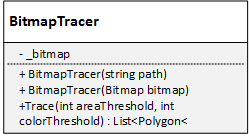
\includegraphics[scale=1.0]{bitmaptracer-class}\\
	\textit{Schemat 1. Klasa BitmapTracer}
\end{center}

~\\Powyższa klasa zawiera jedno pole prywatne - \textit{\_bitmap}, które jest polem oznaczonym modyfikatorem \textit{readonly}. Jest ono inicjalizowane w konstruktorze klasy. Pole to przechowuje obiekt typu \textit{Bitmap}, który będzie podlegał trasowaniu.
\\\\Poza dwoma konstruktorarmi, jedyną i kluczową metodą klasy \textit{BitmapTracer} jest metoda \textit{Trace(int, int)}. Jako parametry przyjmuje ona \textit{area threshold} i \textit{color threshold}, natomiast jako wynik swojej pracy zwraca nam listę rozpoznanych wielokątów.

\section{Trasowanie pliku graficznego}

\subsection{Biblioteka}

Trasowanie odbywa się przy pomocy wrappera zewnętrznej biblioteki \textit{D3DPotrace} będącej dotnetowym portem biblioteki \textit{Potrace}. Jest to jedna z dwóch (obok \textit{AutoTrace}) popularnych bibliotek do trasowania obrazów rastrowych o otwartym kodzie. 
\\\\Działanie samej biblioteki oparte jest na koncepcji hirarchizacji trasowanych obszarów. Przykładowo: umieszczona na białym tle czarna, wypełniona w środku plama jest obszarem traktowanym jako (zamknięty) wielokąt. Jeżeli na takiej czarnej plamie umieścimy całkowicie się w niej zawierającą plamę białą (tworząc czarny obwarzanek), to zostanie ona uznana za potomka plamy czarnej. Jeszcze mniejsza plama czarna zawarta w białej będzie potomkiem białej i pra-potomkiem pierwszej czarnej plamy itd. 
Ponieważ wielokąty zawarte całkowicie w innych wielokątach nie mają żadnego znaczenia (pojazd omijając przeszkodę i tak bierze pod uwagę tylko jej krawędź, a nie jak jest w środku "podziurawiona"), dzięki takiej hierarchizacji danych możemy w łatwy sposób odrzucać wszystkie nieistotne dla obliczenia ścieżki kształty.

\subsection{Wrapper}

Poza odrzucaniem niepotrzebnych figur wrapper ułatwia korzystanie z biblioteki upubliczniając jedynie te parametry, których kastomizacja ma sens. Przykładowo, wrapper ma zakodowany na stałe współczynnik określający w jakim stopniu krawędzie trasowane są do linii beziera zamiast linii prostych. De facto dba o to, żeby krawędzie wyjściowe były wyłącznie odcinkami prostymi.
\\\\Wrapper upublicznia dwa parametry:
\\- Color threshold - procentowa wartość od 0 do 100. Określa stopień w jakim muszą różnić się dwa różnokolorowe fragmenty obrazka, aby zostały zinterpretowane jako dwa różne wielokąty. Przykładowo: mała wartość sprawi, że dwa nachodzące na siebie kwadraty - jeden czerwony, drugi czerwony z niewielką domieszką żółtego - zostaną przetrasowane do dwóch odrębnych obiektów. Duża wartość sprawi, że algorytm zwróci dla tego samego wejścia jeden kształt o polu będącym sumą pól kwadratów - chyba, że kwadraty będą miały zupełnie inne kolory (np. ciemny czerwony i jasny niebieski).
\\- Area threshold - minimalnym pole (de facto ilość pikseli) jakie musi mieć figura, aby nie była zignorowana przez algorytm trasujący. Wartość równa 0 sprawia, że nawet najmniejsze elementy na bitmapie zostaną potraktowane jak wielokąty. Ten parametr może być szczególnie przydatny w celu pozbycia się artefaktów generowanych przez aparat, gdy obrazek wejściowy jest zdjęciem.

\section{Działanie modułu}
	
Użytkownik po wybraniu z menu głównego opcji „Wczytaj plik graficzny” zostaje przeniesiony do odpowiedniego widoku, w którym będzie mógł zdefiniować parametry trasowania a następnie je zrealizować. Bezpośrednio po wejściu do widoku modułu jedynym aktywnym przyciskiem jest przycisk "Wczytaj obraz", po wciśnięciu którego nastąpi otwarcie okna dialogowego i użytkownik będzie miał możliwość wyboru pliku graficznego który ma zostać przetworzony. Ponadto podczas pracy z modułem trasowania, cały czas aktywne pozostają suwaki umożliwiające zmianę parametrów \textit{area threshold} i \textit{color threshold}.

~\\\begin{center}
	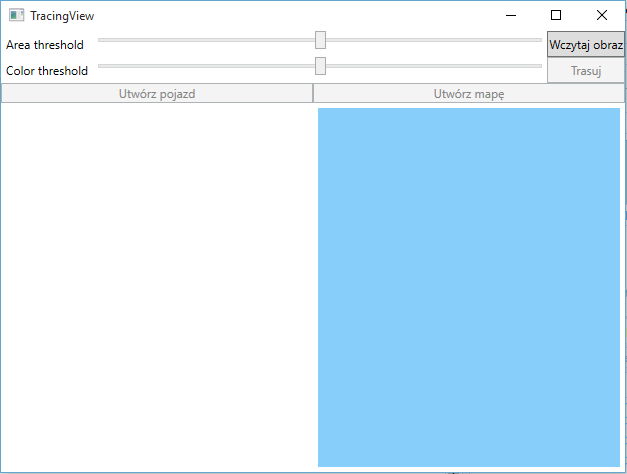
\includegraphics[scale=0.7]{tracingview}\\
	\textit{Rysunek 1. Moduł trasowania}
\end{center}
\newpage
Po wyborze i akceptacji obrazka wejściowego odblokowany zostanie przycisk "Trasuj", po wciśnięciu którego użytkownik będzie mógł zobaczyć wygenerowane kształty. Przykładowe działanie aplikacji zaprezentowano poniżej (po lewej stronie wejściowy obrazek, po prawej stronie wyniki trasowania).

~\\\begin{center}
	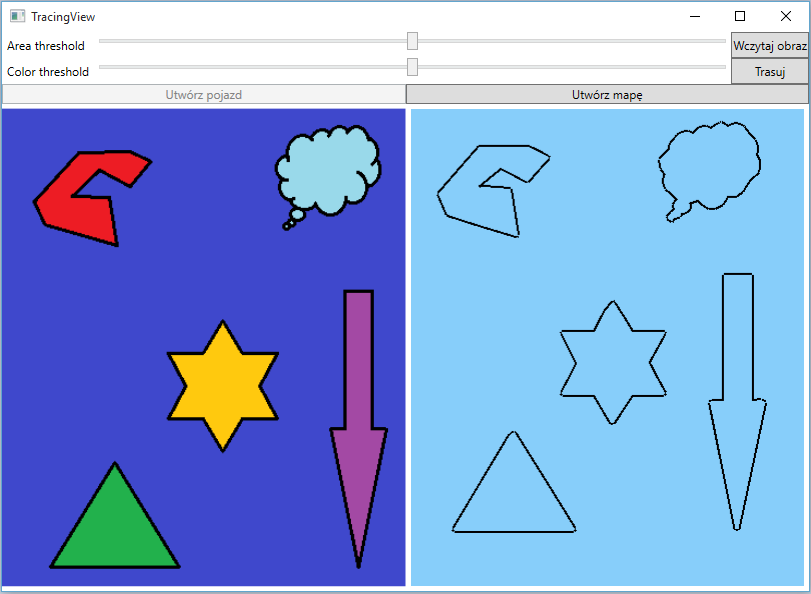
\includegraphics[scale=0.54]{tracingview2}\\
	\textit{Rysunek 2. Przykład trasowania 1}
\end{center}

~\\Jak łatwo zauważyć na powyższym obrazku, aktywowany został przycisk „Utwórz mapę”, natomiast przycisk „Utwórz pojazd” pozostał nadal nieaktywny. Stało się tak dlatego, że wygenerowanych zostało kilka wielokątów. Sytuacja ta jest prawidłowa dla obiektu mapy, gdyż może się ona składać z dowolnej liczby wielokątów będących przeszkodami. Jeśli chodzi zaś o pojazdy, to oczekujemy, że będą się one składać tylko z jednego wielokąta. Konieczne jest więc wskazanie przez użytkownika, który wielokąt chciałby traktować jako kształt pojazdu. Aby to zrobić należy wykonać kliknięcie lewym przyciskiem myszy gdy kursor znajduje się wewnątrz danego wielokąta - zostanie on dodatkowo podświetlony. Gdy wielokąt został już wybrany i nastąpi kliknięcie wewnątrz innego wielokąta, to kształt z którego tworzony będzie pojazd ulegnie zmianie. Wielokąt, który w danej chwili jest kształtem tworzącym pojazd zostanie dodatkowo oznaczony. Po wybraniu wielokąta tworzącego pojazd przycisk "Utwórz pojazd" zostanie odblokowany.
\\\\\\Czasami jednak trasowanie obrazków może dawać zaskakujące efekty i w sytuacji, gdy intuicja podpowiada nam, że powinno powstać kilka wielokątów, powstanie tylko jeden. Wszystko to zależy oczywiście również od odpowiedniego doboru parametrów trasowania. Poniżej zaprezentowano  sytuację, w której z kilku zamkniętych kształtów na obrazku wejściowym powstaje jeden wielokąt.
~\\\begin{center}
	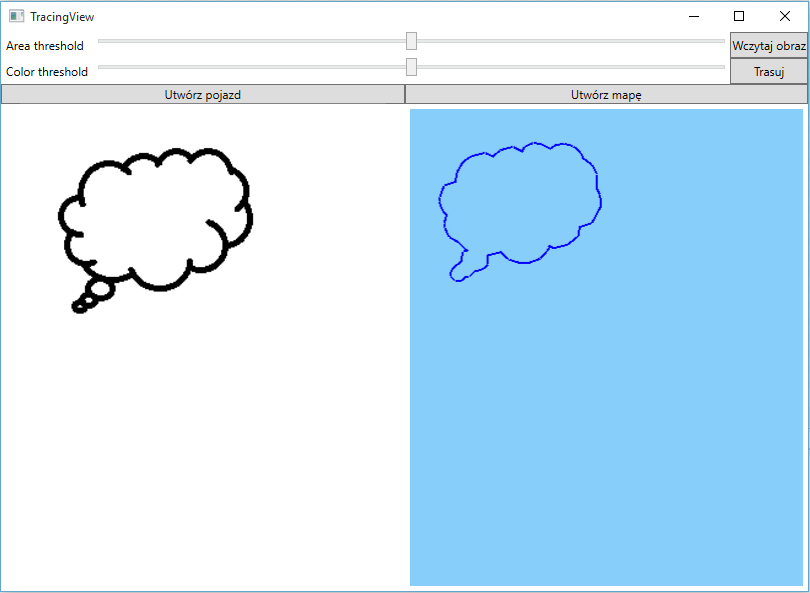
\includegraphics[scale=0.58]{tracingview3}\\
	\textit{Rysunek 3. Przykład trasowania 2}
\end{center}

~\\Dodatkowo warto dodać, iż jeżeli w obrazku wejściowym jakiś wielokąt zawarty jest wewnątrz innego wielokąta, to zostanie on odrzucony. Odrzucenie to odbywa się już na etapie trasowania poprzez wykrywanie potomków. 

\section{Testy}

Dla celów testowych aplikacji napisanych zostało kilka testów sprawdzających poprawność zaimplementowanych metod. Oprócz testowania małych i pomocniczych metod, jak np. metody implementujące proste algorytmy geometryczne, została również przetestowana funkcja trasująca obrazy. Wyniki testów są pozytywne – funkcja trasowania dla różnych obrazów testowych i przy założonych wartościach progowania wygenerowała spodziewane listy wielokątów. Jedynym problemem okazało się generowanie zbyt dużej liczby zbędnych punktów (które leżą na krawędzi wielokąta) dla niektórych przypadków, jednak problem ten zostanie rozwiązany w dalszej części prac nad aplikacją.

\end{document}